% COGNX Technical Report 001, version 0.1, September 2026.
% Empirical source: results/research_benchmark/full/BENCHMARK_REPORT.md.
% Compile from this directory: pdflatex main; bibtex main; pdflatex main; pdflatex main.
\documentclass[10pt,a4paper]{article}
\usepackage[T1]{fontenc}
\usepackage[utf8]{inputenc}
\usepackage{lmodern}
\usepackage[margin=23mm,headheight=14pt]{geometry}


\usepackage{microtype}
\usepackage{amsmath,amssymb}
\usepackage{graphicx}
\usepackage{booktabs,array,tabularx}
\usepackage{tikz}
\usetikzlibrary{arrows.meta,positioning,calc}
\usepackage{caption}
\usepackage[numbers,sort&compress]{natbib}
\usepackage{fancyhdr}
\usepackage{xurl}
\usepackage[hidelinks]{hyperref}
\hypersetup{
  pdftitle={MNEMA: Exploring Fast Associative Memory and Slow Adaptive Learning for Continual Learning},
  pdfauthor={Ujan Dey and Swapnil},
  pdfsubject={COGNX Technical Report 001; version 0.1; not peer reviewed},
  pdfkeywords={continual learning, associative memory, Split-MNIST, technical report}
}
\graphicspath{{figures/}}
\captionsetup{font=small,labelfont=bf,justification=justified}
\pagestyle{fancy}
\fancyhf{}
\fancyhead[L]{\small COGNX Technical Report 001}
\fancyhead[R]{\small MNEMA \textbar\ Version 0.1}
\fancyfoot[C]{\thepage}
\renewcommand{\headrulewidth}{0.3pt}
\setlength{\parskip}{4pt}
\setlength{\parindent}{0pt}
\setlength{\tabcolsep}{5pt}
\renewcommand{\arraystretch}{1.12}
\setlength{\emergencystretch}{2em}
\setlength{\bibsep}{5pt}
\raggedbottom
% Let sections share pages while preventing isolated paragraph lines.
\widowpenalty=10000
\clubpenalty=10000
\displaywidowpenalty=10000
\newcommand{\code}[1]{\texttt{\detokenize{#1}}}
\newcommand{\source}[1]{\par\smallskip{\footnotesize\textit{Repository basis:} #1\par}}

\begin{document}

% Page 1: restrained title page. Page count includes this page.
\begin{titlepage}
\thispagestyle{empty}
{\large COGNX Research \textperiodcentered\ Technical Report 001\par}
\vspace{8mm}
\hrule height 0.5pt
\vspace{38mm}
{\LARGE\bfseries MNEMA: Exploring Fast Associative Memory and Slow Adaptive Learning for Continual Learning\par}
\vspace{18mm}
{\large Ujan Dey\quad and\quad Swapnil\par}
\vspace{4mm}
{\large COGNX Research\par}
\vspace{18mm}
Version 0.1\par
September 2026\par
\vfill
\begin{minipage}{0.92\textwidth}
\textbf{Research status.} This is a technical report, not a peer-reviewed paper.
It describes an experimental NumPy implementation and the completed full
Split-MNIST benchmark preserved in the repository. It does not report a new
training run or claim that MNEMA solves catastrophic forgetting.
\end{minipage}
\vspace{12mm}
\hrule height 0.3pt
\vspace{4mm}
\url{https://github.com/ujandey/mnema}
\end{titlepage}
\setcounter{page}{2}

% Abstract, question, and evidence boundary.
\begin{abstract}
We investigate MNEMA, an experimental architecture combining fast associative
class memory, sparse representations, a slower adaptive spiking projection, and
internal consolidation. This report audits the current repository implementation
and describes its saved full Split-MNIST class-incremental benchmark: five
sequential digit-pair tasks, 60,000 training images, 10,000 test images, six
methods, and ten seeds. All ten classes remain available at inference, without
task-ID masking. Because native MNEMA inference changes adaptive state, the
benchmark restores the trained checkpoint after each test image. In the recorded
results, MNEMA achieves $77.12\pm0.87\%$ final task-macro accuracy and
$6.53\pm1.41$ percentage points of forgetting (mean $\pm$ sample standard
deviation). DER++-300 reaches higher final accuracy, $89.39\pm0.60\%$, whereas
MNEMA has the lowest observed mean forgetting among the six methods. These
metrics must be interpreted together. The nominal 64\,KiB FastStore setting is
not a total-model memory bound: recorded occupied payload is 73,388 bytes and
resident NumPy array payload is 4,391,100 bytes. Inference energy values are
partial operation-counter-based projections. The evidence supports investigation
of a retention--accuracy trade-off under this protocol; it does not establish
statistical significance, broad continual-learning capability, or measured
device efficiency.
\end{abstract}

\section{Introduction}
Continual learning concerns learning from a sequence of experiences while
retaining useful performance on earlier experiences. In a classifier, adapting
shared parameters to later classes can impair recognition of previously learned
classes. Catastrophic forgetting refers to severe interference of this kind;
sequential training need not preserve earlier knowledge simply because a model
has sufficient representational capacity~\citep{mccloskey1989}.

The MNEMA repository investigates an explicit division between rapidly written
associations and slower adaptive learning. Inputs produce sparse addresses used
by both a class-vote memory and a shallow spiking projection. A readout combines
their outputs, while a controller gates learning and periodically transfers
sampled associations into the projection. This is an implemented research
prototype on CPU, with architectural limitations described below, rather than a
demonstrated solution to catastrophic forgetting~\citep{mnemaRepository}.

\textbf{Research question.} Under the repository's sequential Split-MNIST
class-incremental protocol, how does this combination compare with naive
learning, bounded replay, EWC, and DER++ in final accuracy, forgetting, memory
allocation, and projected native inference cost?

The comparison deliberately distinguishes several quantities. Retention after
learning a task is different from how well that task was acquired. Occupied
associative content is different from allocated model state. A native operation
projection is different from an end-to-end measurement. These distinctions are
necessary to interpret the observed strengths and weaknesses of MNEMA.

\subsection*{Scope and evidence}
All empirical results in this report come from the saved full benchmark report,
with its configuration, summaries, plots, and provenance used for cross-checking
and interpretation~\citep{mnemaBenchmark}. Architecture descriptions follow the
current implementation and its audited documentation. Historical experiments
and the one-seed quick run use different protocols and are not pooled with the
full record. Original academic references provide background and algorithm
attribution only; they provide no additional evidence about MNEMA.

The bundle records 60 completed seed--method pairs. Its import audit checked
saved artifacts without rerunning training or inference. The present checkout
is not byte-identical to the recorded benchmark source; Appendix~\ref{sec:repro}
preserves this distinction. The report therefore describes a recorded experiment
and a current implementation audit, not an independent reproduction.

% Architecture and input/fast-memory mechanisms.
\section{Architecture}
\label{sec:architecture}
The entry point is \code{MNEMA.step}. Figure~\ref{fig:architecture} follows the
data and control flow in \code{docs/ARCHITECTURE.md} and \code{mnema/model.py}.
The prediction is formed before the learning operations for that sample.

\begin{figure}[htbp]
\centering
\begin{tikzpicture}[
  font=\small,
  block/.style={draw,fill=white,align=center,minimum height=10mm,text width=27mm,inner sep=3pt},
  smallblock/.style={block,text width=23mm},
  flow/.style={-{Latex[length=2mm]},semithick},
  control/.style={flow,dashed},
  lab/.style={font=\scriptsize,fill=white,inner sep=1pt}
]
\node[smallblock] (x) at (0,0) {Input intensity};
\node[smallblock] (e) at (3.05,0) {E: TTFS encoder};
\node[block] (s) at (6.25,0) {S: sparse separator};
\node[block] (f) at (9.65,1.25) {F: FastStore};
\node[block] (c) at (9.65,-1.25) {C: slow cortex};
\node[smallblock] (r) at (13.05,0) {R: arbitration};
\node[align=center,text width=25mm] (p) at (13.05,-1.6) {Prediction and probabilities};
\draw[flow] (x) -- (e);
\draw[flow] (e) -- (s);
\draw[flow] (s.east) -- ++(0.28,0) |- (f.west);
\draw[flow] (s.east) -- ++(0.28,0) |- (c.west);
\draw[flow] (f.east) -- ++(0.28,0) |- (r.west);
\draw[flow] (c.east) -- ++(0.28,0) |- (r.west);
\draw[flow] (r) -- (p);
% Named endpoints in this lower panel refer to F, C, and R above.
\draw[thin] (-1.2,-2.55) -- (14.25,-2.55);
\node[anchor=west,font=\scriptsize] at (-1.2,-2.9) {Training control and consolidation};
\node[block] (n) at (5,-4.55) {N: controller};
\node[block] (z) at (10,-4.55) {Z: consolidation};
\node[align=center,text width=29mm] (q) at (0.5,-4.05) {F confidence and R prediction};
\node[align=center,text width=29mm] (y) at (0.5,-5.3) {Training label};
\node[align=center,text width=28mm] (fw) at (5,-3.5) {F: write};
\node[align=center,text width=28mm] (cl) at (5,-5.65) {C: learn};
\node[align=center,text width=28mm] (sr) at (13.1,-4.55) {F: sampled rows};
\node[align=center,text width=28mm] (cu) at (10,-3.5) {C: local updates};
\draw[flow] (q.east) -- (n.north west);
\draw[flow] (y.east) -- (n.south west);
\draw[control] (n.north) -- (fw.south);
\draw[control] (n.south) -- (cl.north);
\draw[control] (n.east) -- node[lab,above]{sleep pressure} (z.west);
\draw[flow] (sr.west) -- (z.east);
\draw[flow] (z.north) -- (cu.south);
\end{tikzpicture}
\caption{Current MNEMA data and control flow. Solid arrows carry data or
associations; dashed arrows gate training operations. Named endpoints in the
lower panel refer to the same F, C, and R components shown above. The controller
uses FastStore confidence, the prediction, and an optional training label. Selected
component calls receive software counters (instrumentation is not another
prediction stage). Consolidation samples store rows and updates cortex state.}
\label{fig:architecture}
\end{figure}

\subsection{Input and temporal spike encoder}
For the benchmark, an image has 784 intensity values. Host images are stored as
\code{uint8} and normalized to \code{float32} by division by 255 at use. The
encoder additionally flattens and min--max normalizes its input, with a small
denominator stabilizer. The default time-to-first-spike (TTFS) encoder uses
\textbf{16 bins} and returns a $16\times784$ binary raster. An above-threshold
pixel emits one spike at the clipped value of
$\lceil16(1-x_i^{\mathrm{norm}})\rceil$. Threshold homeostasis runs on every
call. A delta encoder exists, but the model constructor selects TTFS.

\subsection{Sparse separator}
The separator has \textbf{16,384 units}, each with eight fixed, randomly chosen
input connections. Its default top-$k$ selection returns \textbf{64 sparse
indices}. With a reserve fraction of 0.1, selection uses an active pool of
14,745 units; the remaining units are excluded. Adaptive thresholds and running
rates implement homeostasis.

Crucially, the separator first reduces the raster to whether each input spiked
at least once. TTFS timing is therefore collapsed before sparse separation.
The downstream code contains addresses, not a preserved temporal sequence.
Sparse output does not imply that selection and homeostatic computation touch
only 64 units, or that overlap between classes is negligible.

\subsection{FastStore: associative class memory}
FastStore maintains a dense $16{,}384\times10$ array of \code{int16} class
weights, plus per-row salience and timestamps. For selected indices $I$, its
score for class $d$ is $f_d=\sum_{i\in I}M_{i,d}$. Confidence is the gap between
the two largest scores divided by the absolute largest score plus $10^{-5}$.
Writes increment the target-class weights and row salience; budget enforcement
evicts low-salience rows. These are shared address--class associations, not a
buffer of complete examples. Section~\ref{sec:memory} separates their active
content from allocated capacity.
\source{\code{mnema/model.py}, \code{encoder.py}, \code{separator.py}, and
\code{store.py}; recorded initial settings in \code{config.json}.}

% Architecture continued.
\subsection{Slow cortex and adaptive synapses}
The cortex is a \textbf{single adaptive spiking projection} from the sparse
representation to ten output units. The constructor stores a
\code{hidden_dim=256} argument, but it does not instantiate a hidden layer.
Four coupled \code{float32} synaptic state planes of shape
$4\times10\times16{,}384$ provide Benna--Fusi-inspired memory variables; only
the first plane is the visible weight matrix~\citep{benna2016}.
This attribution does not imply that MNEMA establishes the theoretical
retention or scaling properties of that work.

At each forward call, the cortex gathers the active columns of the visible
weight matrix and sums them into ten synaptic inputs. It updates leaky membrane
voltages, compares them with adaptation-dependent thresholds, resets firing
units, and updates adaptation. The returned cortex score is the
\emph{post-reset membrane voltage}, rather than a class spike count or a deep
network output. One such update consumes the sparse code; the encoder's
16-bin raster is not propagated through 16 cortex time steps.

During training, eligibility traces decay and accumulate a local surrogate
derivative on active columns. When the overall prediction is incorrect, the
cortex forms the local update
\begin{equation}
  \Delta W_{d,i}=\eta\,(\mathbf{1}[d=y]-v_d)\,e_{d,i},
  \qquad \eta=10^{-3},
\end{equation}
where $v_d$ is its membrane score and $e_{d,i}$ the eligibility trace. The
update enters the first synaptic plane, followed by sequential coupled
diffusion between planes. Trace decay, weight-update construction, and
diffusion include dense array operations. The architecture thus combines
sparse gathering with substantial adaptive state and dense learning work.

\subsection{Readout and arbitration}
Let $f$ be FastStore scores, $c$ cortex membrane scores, and $q$ FastStore
confidence. Cortex familiarity is $h=\max(c)-\operatorname{mean}(c)$. With
the default coefficients, arbitration computes
\begin{equation}
 a=\operatorname{sigmoid}\!\left(\operatorname{clip}(2q-h,-10,10)\right),
 \qquad p=\operatorname{softmax}\!\left(af+(1-a)c\right).
\end{equation}
The class prediction is $\arg\max_d p_d$. Fast and slow pathways are therefore
combined at inference. The readout's stored \code{a2} parameter is unused in
the current computation; the presence of that parameter does not establish
another gating mechanism.

\subsection{Neuromodulatory controller}
The controller computes novelty $\nu=\max(0,1-q)$, a binary prediction error
$\delta$ when a label is available, and accumulated sleep pressure
$\phi\leftarrow\phi+\nu+\delta$. When training is enabled and a label is
present, $\nu>0.15$ triggers a FastStore write, $\delta>0$ triggers cortex
learning, and $\phi\geq50$ triggers consolidation followed by a pressure
reset. The named surprise field \code{sigma} is unused. These implemented
signals should not be interpreted as a validated biological controller or an
implemented surprise-dependent learning-rate schedule.

\subsection{Consolidation}
Each consolidation invocation samples up to 64 occupied FastStore rows without
replacement, with sampling probabilities proportional to
$\mathrm{salience}^{0.6}$. The largest class weight supplies a target label.
For each row, the consolidator constructs a \textbf{single-index activation},
resets cortex neuron and eligibility state, and performs a forward call and
local learning update. It decreases that row's salience by two and clears its
class weights if salience reaches zero.

This mechanism transfers sampled associations toward cortex. It does not replay
the original 64-index pattern, reconstruct an image, or preserve complete
historical codes. The full comparison does not isolate the causal contribution
of consolidation; evaluating that contribution requires ablations.
\source{\code{mnema/cortex.py}, \code{readout.py}, \code{modulators.py},
\code{consolidate.py}, and \code{docs/ARCHITECTURE.md}~\citep{mnemaRepository}.}

% Protocol, algorithms, and metrics use normal body spacing and page flow.
\section{Experimental Protocol}
\label{sec:protocol}
\subsection{Split-MNIST class-incremental learning}
The full benchmark uses $01\rightarrow23\rightarrow45\rightarrow67\rightarrow89$,
60,000 training images, 10,000 test images, and seeds 0--9 for each of six
methods. Methods share each seed's shuffled training indices, presenting every
example once externally. All five test tasks, including future tasks, are
evaluated after each training task. Inference considers \textbf{all ten classes},
without task IDs, output masking, or task-specific heads~\citep{mnemaBenchmark}.

\subsection{Compared methods}
Dense baselines share a $784\rightarrow256$ ReLU $\rightarrow10$ \code{float32}
MLP, identical initialization per seed, and SGD at learning rate 0.01, without
momentum or pretraining. Defaults are fixed, without validation-based
hyperparameter search or final-test-set tuning.

\textbf{Naive MLP} updates on each incoming example's cross-entropy (CE).
\textbf{Replay-300} (``Replay-300 (Research)'' in the artifacts) stores 300
\code{uint8} images and labels in a true reservoir. When nonempty, it draws one
prior example before insertion and updates on mean current-plus-replay CE.
\textbf{Replay-64KiB} uses the same policy with a strict 65,536-byte allocated
buffer budget including images, labels, and size/seen counters: 83 images.
This is not exact total-memory matching with MNEMA.

\textbf{EWC} uses a task-wise diagonal Fisher penalty ($\lambda=100$), with
separate past-task snapshots and Fishers~\citep{kirkpatrick2017}. Its empirical
Fisher averages squared per-example CE gradients using observed labels. All
training examples of the first four tasks are reread without optimizer updates;
no final-task Fisher is built. EWC receives training task boundaries and makes
additional data accesses.

\textbf{DER++-300} stores 300 images, labels, and ten \code{float32} logits
captured before the original optimizer update. Its loss is current CE plus
$0.5$ times mean squared logit error plus $0.5$ times replay-label CE.
Independent prior examples supply the replay terms in one combined
update~\citep{buzzega2020}. \textbf{MNEMA} uses the defaults in
Section~\ref{sec:architecture}, including consolidation. One external pass
does not equalize rehearsal, Fisher-estimation, or consolidation compute.

\subsection{Checkpoint-isolated MNEMA evaluation}
Native \code{is_training=False} skips learning and eligibility maintenance but
changes encoder threshold, separator homeostasis, cortex membrane/adaptation,
and controller state. Predictions can depend on earlier inputs. The research
adapter restores inference-mutable state and RNG state in \code{finally} after
every test image, including exceptions. It preserves the checkpoint's existing
membrane state rather than zeroing it. Predictions receive no labels or task IDs.
Full attribute-state hashes are checked before/after each evaluation set;
final-checkpoint MNEMA predictions are also checked in reverse order, image by
image. Isolation belongs to \textbf{the evaluation protocol}, not native inference.

\subsection{Metrics and replication}
Let $R_{t,j}$ be task-$j$ accuracy as a fraction after learning task $t$, with
zero-based indices $0,\ldots,4$. The reported quantities are
\begin{align}
 \mathrm{ACC}_{\mathrm{final}}&=\frac{100}{5}\sum_{j=0}^{4}R_{4,j},\label{eq:acc}\\
 \mathrm{F}&=\frac{100}{4}\sum_{j=0}^{3}
 \left(\max_{t\in\{j,\ldots,3\}}R_{t,j}-R_{4,j}\right).\label{eq:forget}
\end{align}
Accuracy is a task-macro average, not pooled image accuracy. Forgetting is in
percentage points (pp); its maximum excludes pre-learning and final
checkpoints, and the fifth task is omitted. Negative forgetting is allowed.
Means and sample SDs use the seed as the unit of replication ($n=10$,
\code{ddof=1}); SD is not standard error or a confidence interval.
\source{Full benchmark report/configuration; evaluation, metrics, and runner
in \code{experiments/}; research methods in \code{baselines/}.}

% Original results and retention plot.
\section{Results}
\label{sec:results}
Table~\ref{tab:results} reproduces the full benchmark's reported values.
All uncertainties on accuracy and forgetting are sample SDs across ten seeds.
The reported mean rankings are descriptive; no statistical-significance claim
or claim of optimal algorithm tuning follows from this comparison.

\begin{table}[htbp]
\centering
\caption{Full Split-MNIST comparison, transcribed from
\code{BENCHMARK_REPORT.md}~\citep{mnemaBenchmark}. Accuracy and forgetting are
mean $\pm$ sample SD. Memory and inference projections are reported means.
The projection is partial native inference cost, not measured device energy.
Replay-300 abbreviates the artifact's ``Replay-300 (Research)''.}
\label{tab:results}
\small
\begin{tabularx}{\textwidth}{@{}Xrrrr@{}}
\toprule
Method & Final ACC (\%) & Forgetting (pp) & Resident arrays (B) &
\shortstack{Projected inference\\($\mu$J/image)}\\
\midrule
Naive MLP   & $19.79\pm0.06$ & $99.52\pm0.12$ & 814,120   & 1.768\\
Replay-300  & $82.44\pm1.33$ & $20.58\pm1.62$ & 1,049,636 & 1.768\\
Replay-64KiB& $67.59\pm2.07$ & $39.30\pm2.60$ & 879,291   & 1.768\\
EWC         & $19.98\pm0.36$ & $99.12\pm0.40$ & 7,327,080 & 1.768\\
DER++-300   & $89.39\pm0.60$ & $12.12\pm0.73$ & 1,061,636 & 1.768\\
MNEMA       & $77.12\pm0.87$ & $6.53\pm1.41$  & 4,391,100 & 0.316\\
\bottomrule
\end{tabularx}
\end{table}

DER++-300 achieves the highest observed mean final accuracy. Both DER++-300
and Replay-300 exceed MNEMA's accuracy, by 12.27 and 5.31 pp respectively in
the source report. MNEMA exceeds Replay-64KiB's final accuracy by the reported
9.54 pp and has the lowest observed mean forgetting among these six methods.
These observations apply to the declared protocol and memory boundaries.

\begin{figure}[htbp]
\centering
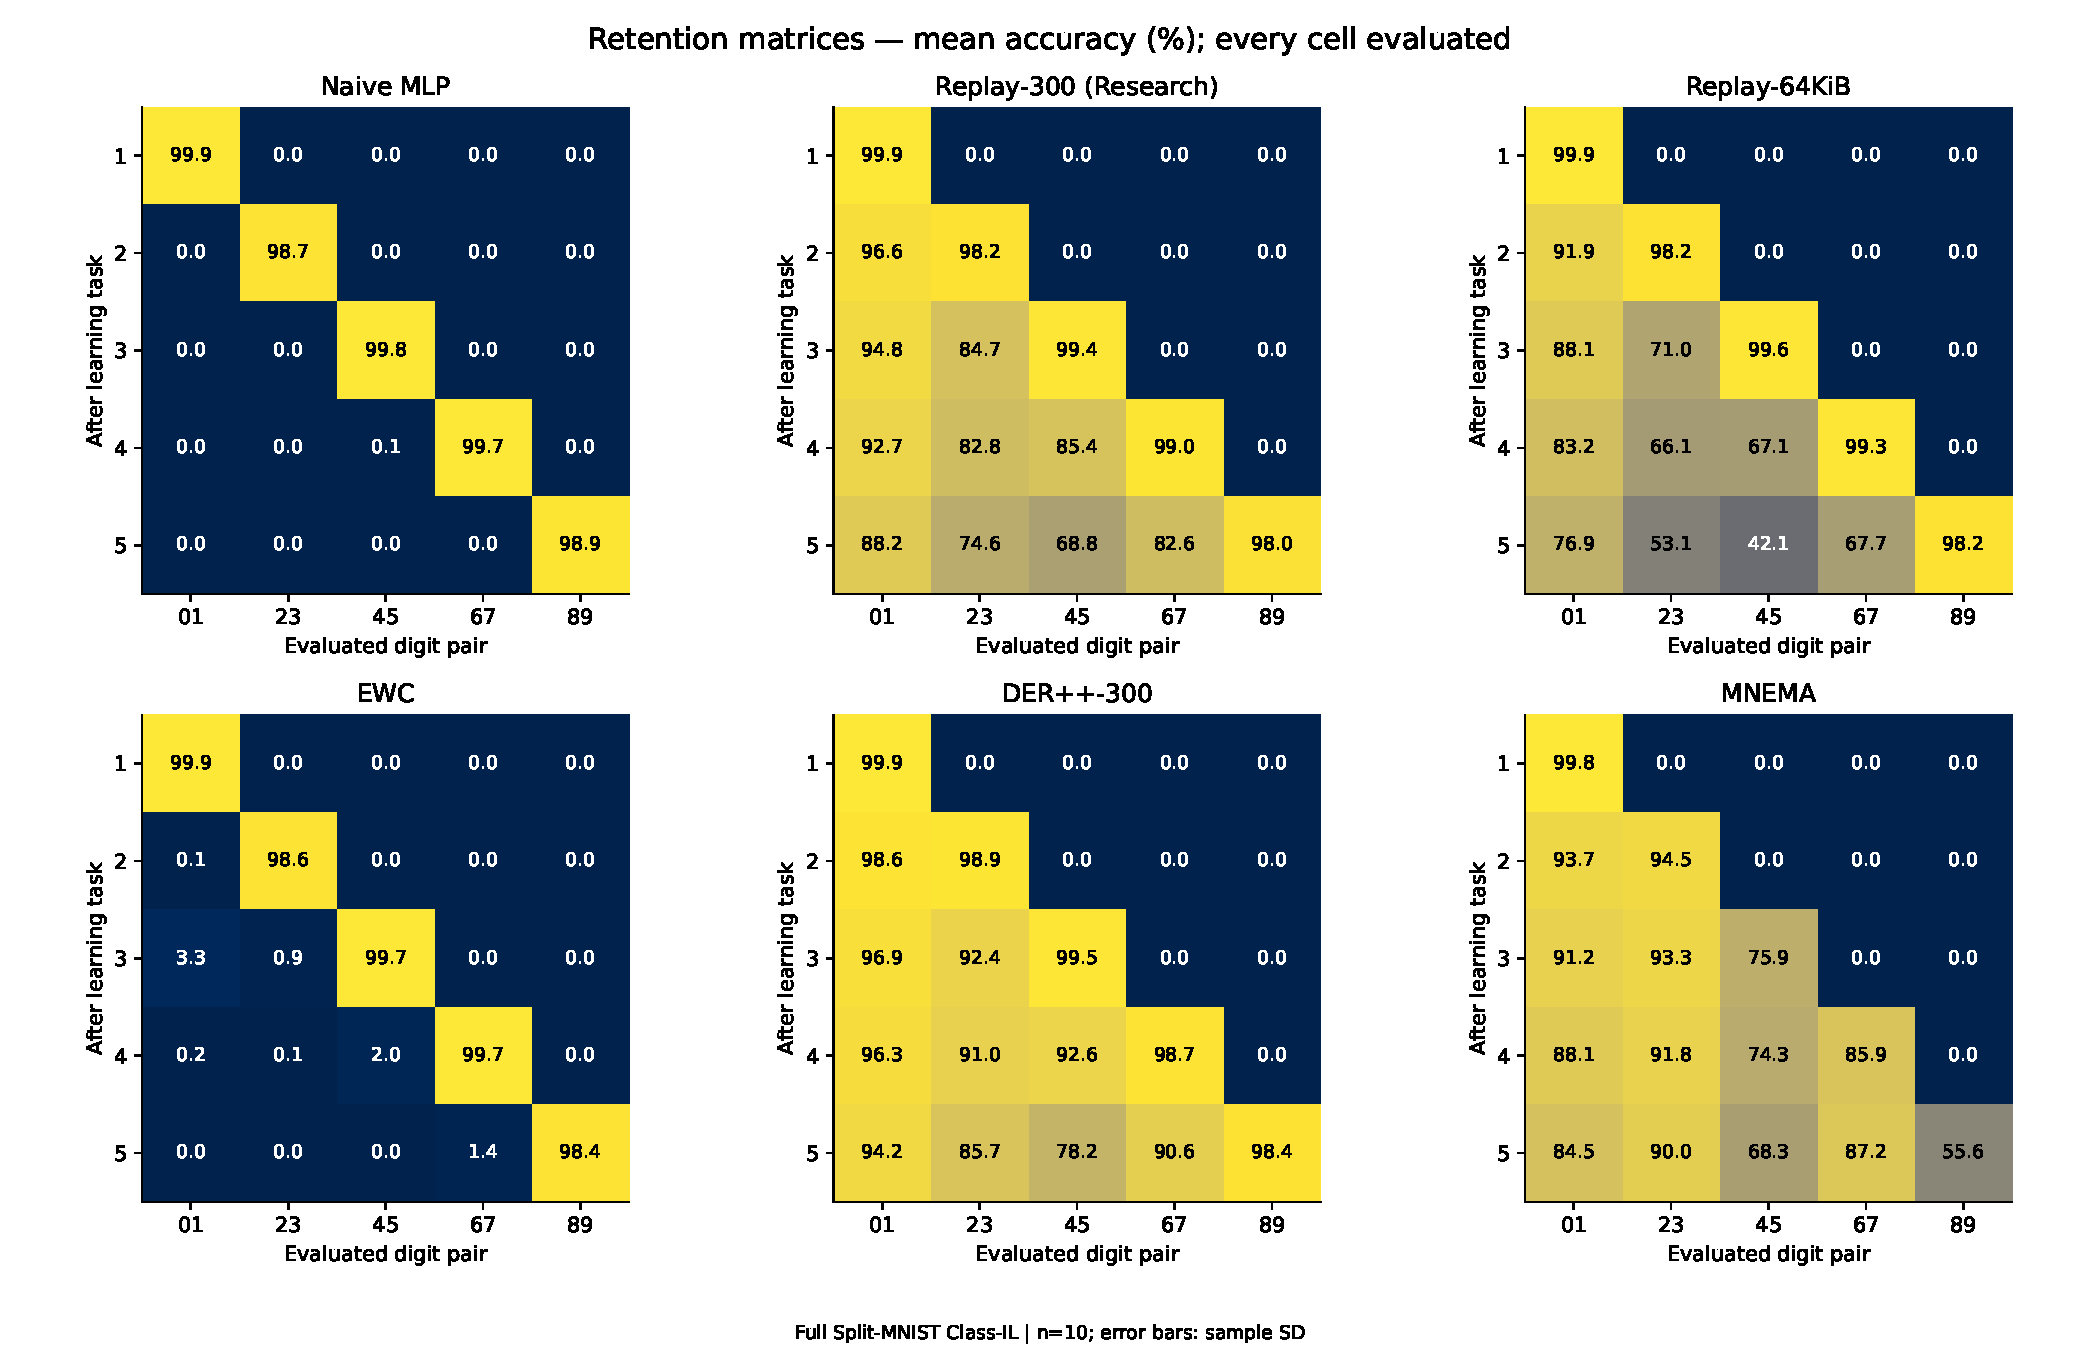
\includegraphics[width=\textwidth]{retention_matrices.pdf}
\caption{Original full-benchmark retention matrices, copied without alteration
from \code{plots/retention_matrices.pdf}~\citep{mnemaBenchmark}. Rows are
post-training checkpoints and columns evaluated digit pairs; cells are mean
accuracy (\%) over ten seeds. All cells, including future-task cells, were
evaluated. The inherited footer mentions error bars generically, but these
heatmaps show means only. Forgetting is computed per seed using
Equation~\eqref{eq:forget}, not from the rounded displayed means.}
\label{fig:retention}
\end{figure}

Accuracy and forgetting answer different questions. A small decrease from a
previously attained score can coexist with incomplete task acquisition or low
final performance. Figure~\ref{fig:retention} makes the distinction visible;
the forgetting ranking alone cannot establish the best final classifier.
The record supports a retention--accuracy trade-off, rather than a general
ordering of continual-learning algorithms.

% Accounting with all categories from the original table.
\section{Memory and Efficiency}
\label{sec:memory}
\subsection{Memory boundaries}
The benchmark counts unique persistent NumPy array payload. Total resident
arrays equal model/adaptive state plus fixed scaffold plus allocated auxiliary
state. Active auxiliary content is an alternative occupancy view and is not
added again. Python object and scalar overhead, PRNG internals, shared dataset
arrays, temporary gradients/Fisher workspace, and evaluation snapshots are
excluded for all methods. These values are neither process RSS nor peak RAM.
Buffer seen/size counters are explicit \code{int64} arrays and are included.

\begin{table}[htbp]
\centering
\caption{Final array-payload decomposition in bytes, from the full benchmark
report. All entries are reported means with sample SD zero. Total resident
payload in Table~\ref{tab:results} is adaptive + fixed + auxiliary allocated;
auxiliary content must not be counted twice.}
\label{tab:memory}
\small
\begin{tabularx}{\textwidth}{@{}Xrrrr@{}}
\toprule
Method & Model/adaptive & Fixed scaffold & Aux. content & Aux. allocated\\
\midrule
Naive MLP    & 814,120   & 0       & 0         & 0\\
Replay-300   & 814,120   & 0       & 235,516   & 235,516\\
Replay-64KiB & 814,120   & 0       & 65,171    & 65,171\\
EWC          & 814,120   & 0       & 6,512,960 & 6,512,960\\
DER++-300    & 814,120   & 0       & 247,516   & 247,516\\
MNEMA        & 3,408,032 & 524,316 & 73,388    & 458,752\\
\bottomrule
\end{tabularx}
\end{table}

MNEMA's adaptive allocation includes cortex synaptic planes, eligibility
traces, neuron arrays, and separator homeostasis. The fixed scaffold includes
separator connectivity and synaptic constants. The memory advantage of small
occupied associative content cannot be extended to the whole implementation.

\subsection{Configured FastStore budget versus actual payload}
The configured budget is 65,536 bytes (64\,KiB, with 1\,KiB = 1,024 bytes).
Eviction counts $10\times2+5=25$ bytes per occupied row. The actual row payload
is $10\times2+4+4=28$ bytes: ten \code{int16} weights, \code{float32}
salience, and a \code{uint32} timestamp. Table~\ref{tab:faststore} reports the
resulting discrepancy. All store arrays remain densely allocated.

\begin{table}[htbp]
\centering
\caption{FastStore configuration and recorded final occupancy. Values are
identical across the ten seeds in the full report (sample SD zero). Occupancy
and allocated capacity have different meanings.}
\label{tab:faststore}
\small
\begin{tabularx}{0.92\textwidth}{@{}Xr@{}}
\toprule
Quantity & Value\\
\midrule
Configured FastStore budget (B) & 65,536\\
Implementation / actual bytes per occupied row & 25 / 28\\
Occupied rows & 2,621\\
Implementation-counted occupancy (B) & 65,525\\
Actual occupied payload (B) & 73,388\\
Allocated FastStore arrays (B) & 458,752\\
Total MNEMA resident NumPy array payload (B) & 4,391,100\\
\bottomrule
\end{tabularx}
\end{table}

The full report records 597,911 post-sample over-budget observations across
the ten MNEMA runs. Monitoring follows each external training sample and its
consolidation; the recorded maximum is not a bound on within-step transients.
Occupied payload also does not demonstrate a packed sparse deployment format,
which could require additional address metadata.

\subsection{Operation-counter-based energy projections}
The saved inference estimates use \code{instrument/tech/asic_45nm.yaml}.
Selected software counters are multiplied by technology-card coefficients;
\code{project_energy()} marks the result \code{is_measured=False}. The reported
means are 0.316\,$\mu$J/image for MNEMA and 1.768\,$\mu$J/image for each dense
baseline. Coverage is incomplete: the projection does not charge recorded
write traffic, portions of arithmetic, or checkpoint restoration. The selected
card has no synaptic-operation or neuron-update coefficients. A smaller
projection therefore does not establish a physical deployment advantage.
\source{Full report, Sections 4, 7, and 8; \code{experiments/research_memory.py};
\code{instrument/counters.py} and the selected technology card.}

% Balanced discussion and original auxiliary-memory plot.
\section{Discussion}
\subsection{Where MNEMA performs well}
MNEMA's observed mean forgetting is lower than that of all five alternatives
in this record. At the same time, its final accuracy exceeds Naive MLP, EWC,
and Replay-64KiB. The results suggest that the current combination of
associations, adaptive state, and consolidation merits further investigation
as a way to retain useful classification behavior during this task sequence.
They do not identify which component is responsible for the observation.

The comparison with Replay-64KiB is informative but requires precise memory
language. MNEMA has higher final accuracy and lower mean forgetting, while its
occupied FastStore payload exceeds that baseline's allocated episodic buffer,
and its total resident state is substantially larger. The comparison cannot
be described as superiority at an equal 64\,KiB model budget.

\begin{figure}[htbp]
\centering
{\scriptsize\bfseries x-axis is not total resident memory\par}
\vspace{2pt}
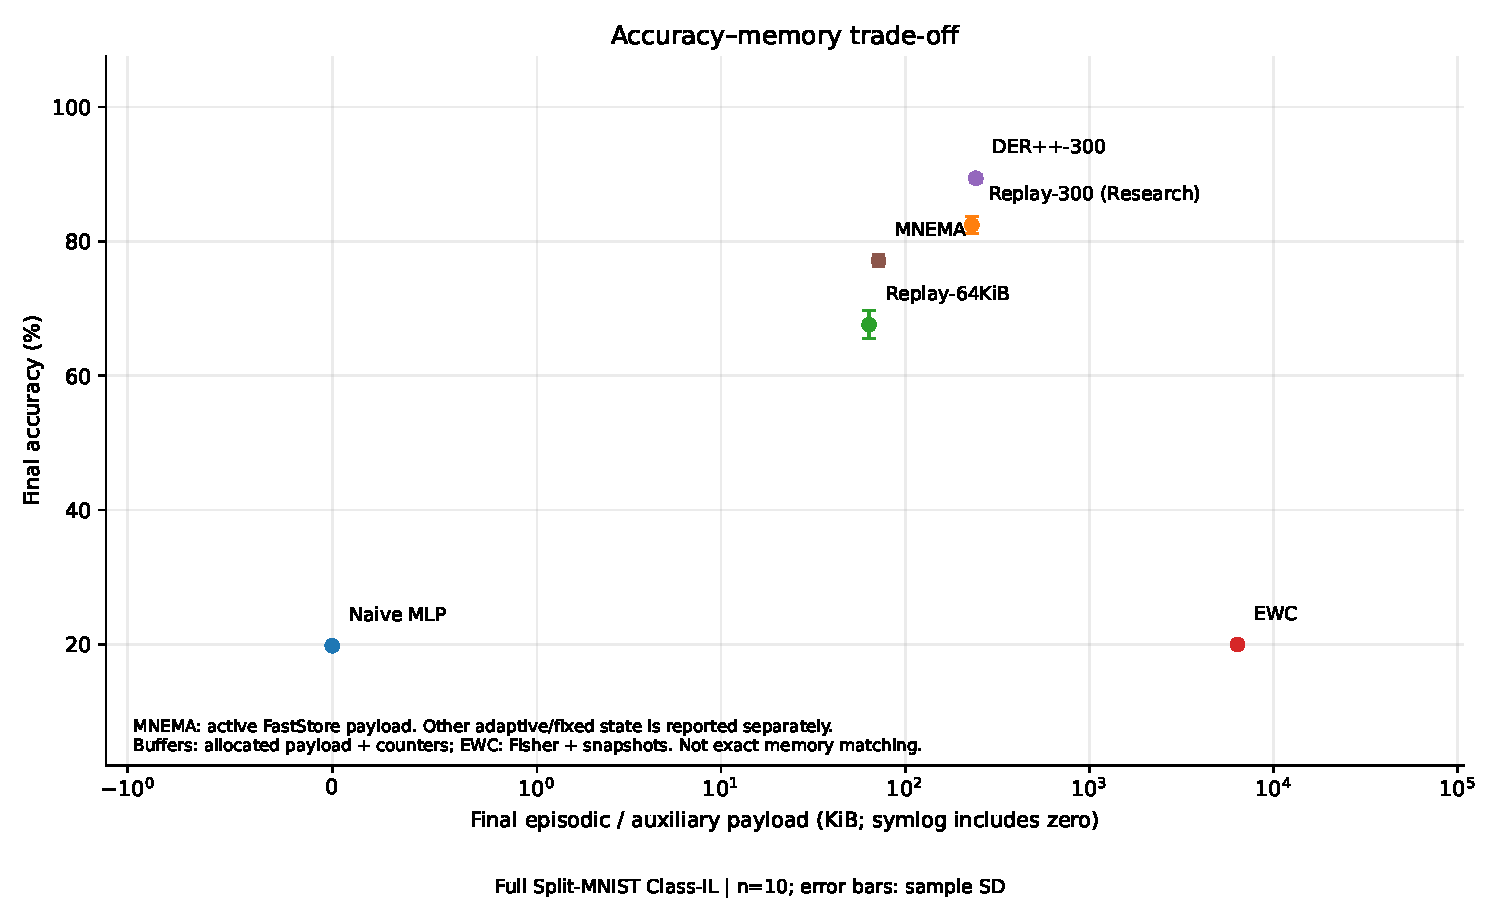
\includegraphics[width=0.94\textwidth]{accuracy_vs_memory.pdf}
\caption{Original full-benchmark accuracy versus \emph{auxiliary} payload,
copied unchanged from \code{plots/accuracy_vs_memory.pdf}. Despite broader
descriptions elsewhere in the repository, its horizontal axis is not total
resident model memory. MNEMA uses occupied FastStore payload, replay methods
use allocated buffers and counters, and EWC uses Fishers and snapshots.
Error bars show sample SD across ten seeds; the horizontal scale is symmetric
logarithmic to include zero. Read with Tables~\ref{tab:results}
and~\ref{tab:memory}, which expose additional resident allocation.}
\label{fig:auxmemory}
\end{figure}

\subsection{Where MNEMA performs poorly}
\textbf{Replay-300 and DER++-300 both achieve higher final accuracy than
MNEMA and use less total resident NumPy array payload.} This is a material
negative result for the current architecture. EWC uses more resident state
than MNEMA, so the memory comparison is method-dependent rather than universal.
The low-forgetting observation does not reverse the final-accuracy ordering.

Several implementation realities limit interpretation. The cortex is shallow;
temporal information is lost before sparse separation; consolidation trains on
individual row associations; and store eviction does not enforce the configured
budget against actual payload. These are reasons to test targeted changes,
not established causal explanations for the accuracy deficit. The full
benchmark is not an ablation study.

Efficiency comparisons have a further boundary. MNEMA's sparse gathering does
not remove dense eligibility and synaptic-diffusion work during learning.
Baseline training, buffer operations, and Fisher estimation lack comparable
complete energy instrumentation. No cross-method training-energy ranking is
supported. Host wall-clock time, which includes integrity work, cannot be
converted into measured energy by assertion. Technology-card projections
provide a partial accounting model, not evidence of neuromorphic deployment.

% Limitations, proposed next experiments, modest conclusion.
\section{Limitations}
\label{sec:limitations}
\textbf{Dataset and protocol coverage.} The evidence is limited to MNIST,
one fixed digit-pair order, and ten seeds. It does not establish performance
on other visual domains, alternative orders, longer streams, or broader
continual-learning settings. All outputs remain available at inference, but
training uses known task partitions and EWC receives task boundaries.

\textbf{Architecture and tuning.} Model scale is limited, with simple dense
baselines and a shallow MNEMA cortex. Hyperparameters are fixed rather than
selected through a validation-based search. Poor EWC performance here is not
evidence against every EWC configuration. TTFS timing is collapsed before
sparse separation. Single-row consolidation differs from complete-example
replay. No full-protocol component ablations establish the contribution of
FastStore, cortex, arbitration, or consolidation individually.

\textbf{Stateful inference.} Native inference changes adaptive state.
Checkpoint isolation is a benchmark convention, not native statelessness.
The report therefore evaluates predictions from a fixed trained state per
image, not unrestricted sequential test-time adaptation. Restoring the
checkpoint's membrane state also differs from zero-state inference.

\textbf{Memory and compute accounting.} The FastStore row-size discrepancy
prevents a true 64\,KiB active-payload bound. Total resident NumPy state is
larger than for the replay baselines, and array payload omits runtime overhead
and temporary workspace. A single external training pass does not equalize
computation: EWC performs extra Fisher reads, and replay methods and MNEMA
perform internal rehearsal. There is no common compute-budget control.

\textbf{Energy and deployment.} Energy is projected from incomplete counters,
not measured on a device. Uncharged writes, omitted arithmetic, dtype/traffic
assumptions, and excluded evaluation restoration limit the estimates. No
neuromorphic hardware deployment or end-to-end physical energy comparison is
reported.

\textbf{Statistical and provenance scope.} Mean and sample SD do not establish
statistical significance. Seed replication does not replace dataset and
task-order replication. The saved bundle passes its recorded artifact checks,
but current-source differences preclude claiming exact reproduction from this
checkout; cross-platform floating-point identity is not guaranteed. These
results do not establish that MNEMA solves catastrophic forgetting.

\section{Future Work}
The following are proposed follow-up studies, \textbf{not completed results}
in the audited full benchmark. The repository explicitly identifies
Split-FashionMNIST as the next dataset. Multiple task orders and stronger
continual-learning datasets would test whether the observed trade-off extends
beyond the present sequence. Such runs should retain declared inference
semantics, held-out selection, and separate provenance.

The FastStore accounting discrepancy should be corrected and evaluated in a
new experiment, preserving the existing evidence. Future memory accounting
should distinguish actual occupied content, allocation, address metadata,
temporary workspace, and peak process memory. A stricter budget would change
capacity and could change performance; its outcome cannot be inferred from
the present table.

Architecture studies should compare FastStore-only, cortex-only, and
no-consolidation variants under the same evaluation protocol, alongside
ablations of arbitration, sparse-code parameters, and adaptive synaptic state.
Preserving temporal information beyond the encoder would directly address the
current timing collapse. These are proposed tests of mechanisms, not claims
that a particular change will improve accuracy or retention.

More complete operation instrumentation and comparable compute reporting
should precede eventual neuromorphic or other hardware evaluation. Actual
deployment studies would need measured device behavior and implementation
costs, rather than interpreting a different technology card as a hardware run.

\section{Conclusion}
MNEMA is an experimental exploration of fast associative memory with slower
adaptive learning and consolidation. In the saved full Split-MNIST protocol,
it has the lowest observed mean forgetting, while Replay-300 and DER++-300
achieve higher final accuracy with less resident array payload. The useful
next step is to test the mechanisms and accounting boundaries explicitly.
The present evidence supports that investigation without establishing a
general solution to catastrophic forgetting.

% Reproducibility and bibliography.
\appendix
\section{Reproducibility and Evidence Map}
\label{sec:repro}
Repository: \url{https://github.com/ujandey/mnema}.
Run the full benchmark from the repository root:
\begin{quote}\small\ttfamily
python experiments/run\_research\_benchmark.py --mode full --seeds 10
\end{quote}
This command executes all 60 seed--method pairs sequentially. The saved run
used independent CPU workers on GitHub Actions. Its September 11, 2026
configuration records Python 3.11.7, NumPy 2.2.6, Matplotlib 3.10.3,
PyYAML 6.0.2, and one BLAS thread. Use the standalone pins in
\code{experiments/research_requirements.txt}, not the separate Python 3.14
package environment.

\textbf{Recorded benchmark source commit:}\par
\nolinkurl{fe86ec1c6abc600dda8ec50565a551af4e5434bd}

The full report, configuration, raw results, per-seed indices, summaries,
plots, checksums, and worker records are preserved under
\code{results/research_benchmark/full/}. The import audit checked saved
artifacts without rerunning training or inference. The audited checkout
differs from the recorded source, so exact-source reproduction requires that
source and environment. New experiments should preserve the existing bundle
in a separate checkout/output context.

\code{BENCHMARK_REPORT.md} is the empirical authority. Architecture and
evaluation follow the repository documentation and implementation. The
accompanying report README retains the detailed source map, checkout identity,
figure checksums, and reproduction caveats. Preparing this report changed
neither research code nor benchmark data.

\begingroup
\small
\bibliographystyle{unsrtnat}
\bibliography{references}
\endgroup
\end{document}
